\documentclass{article}

\usepackage{graphicx}

\begin{document}
\section*{Description of problem}
\noindent Here's a short description of what's done: \\
For each frame from movie I've converted it to grayscale, used guassian blur on the image to remove some noise.\\
Adaptive threshold to find binary image.\\
Erode and dilate to remove too small objects.\\
Hough transform to find the circle in the image.\\
Write the coordinates of the center and which frame and time it was found.\\

\noindent I've also tried to use Otsu's for the thresholding and then shape recogonition. Where I checked the roundness of the shapes after otsu's but it seems to have a high frame loss. From what I could tell most of the lost frames are when the circle is close to the edge of the screen.\\

\noindent Is there any better way to do the thresholding for these images that would be stable for the different lightning conditions? \\

\noindent Here's some graphs for describing the problem. The blue and green graphs are with hough transform and shape recognition. Both have alot of missing frames. For the first half there's an animated dot moving at various speeds and then standing still for a brief period. Around 85 seconds in theres a small break between tests until 90 seconds where there's a stationary test with dots appearing and reappearing at various locations with no animation. \\

\noindent 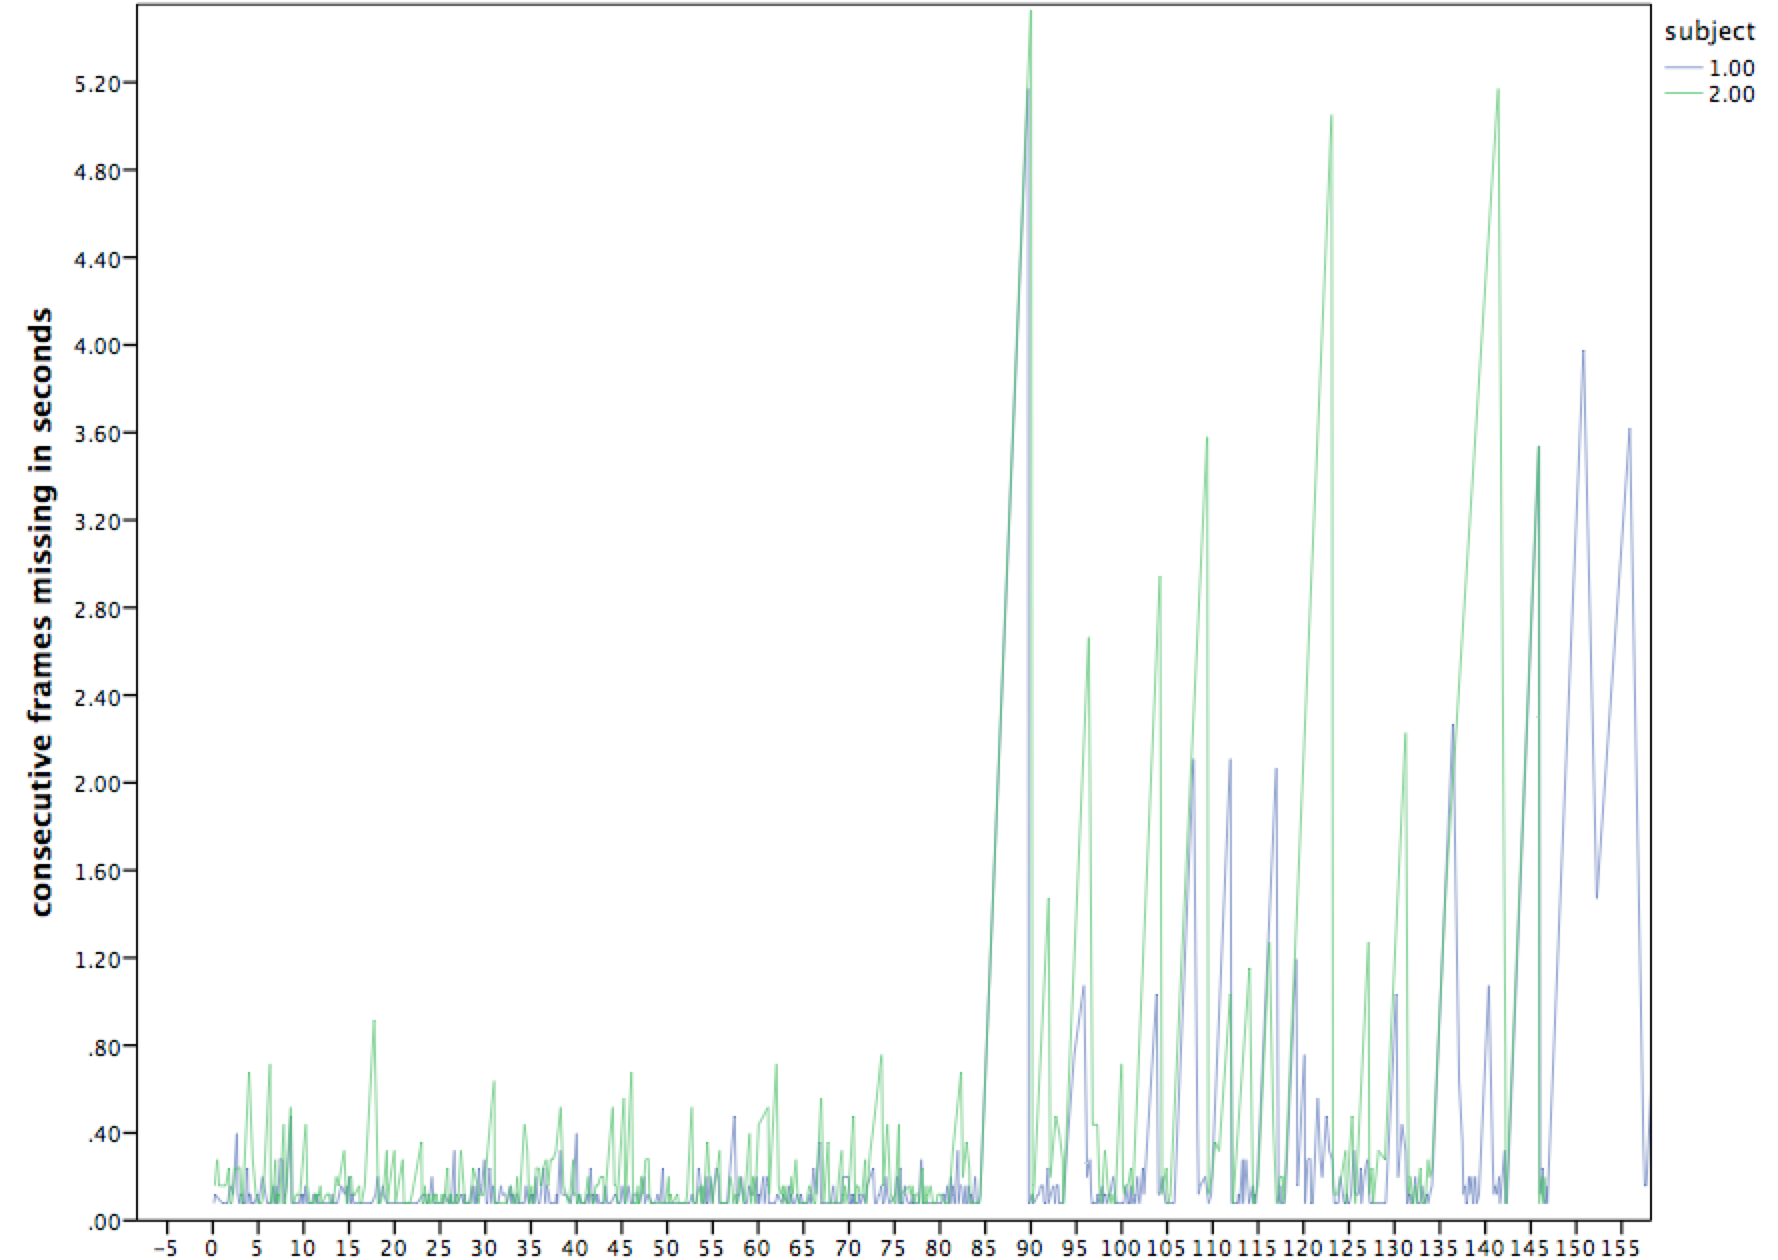
\includegraphics[scale=0.4]{./img/consec_frames_full.png}

10 least lossy seconds during the first half still have a lot of consecutive frame loss, often up to 40\% or 50\%.\\

\noindent 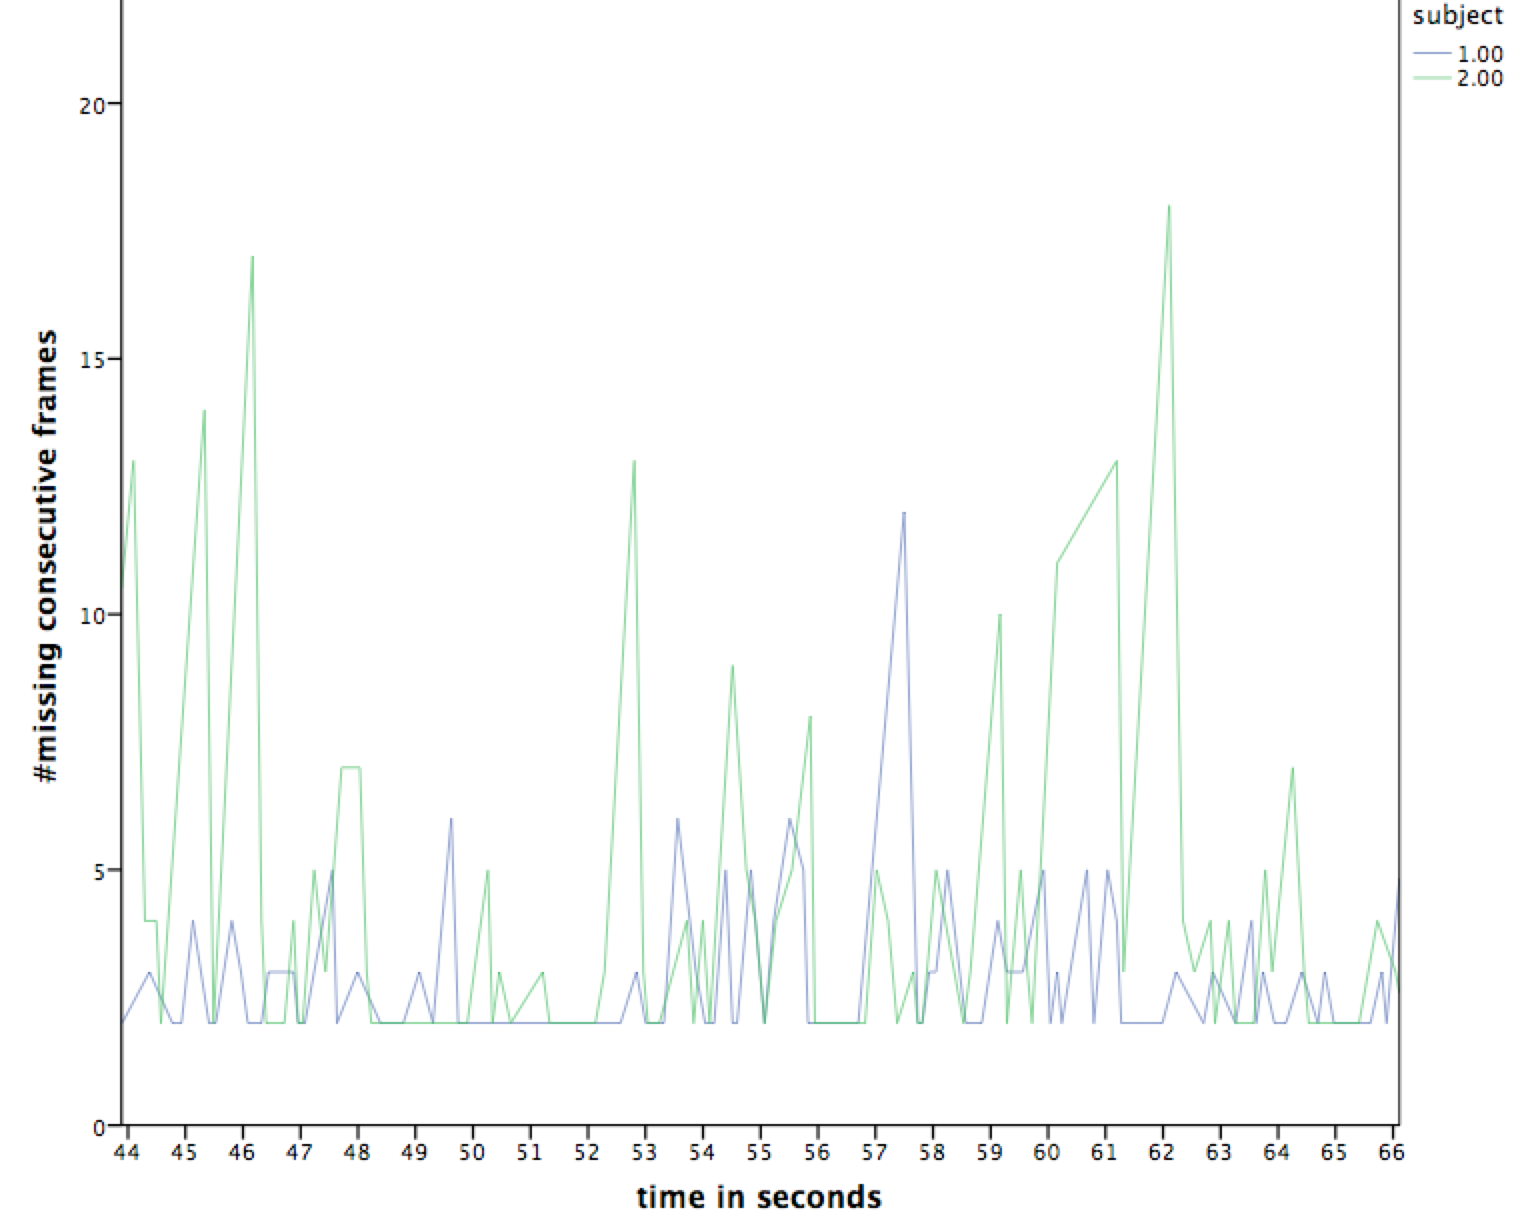
\includegraphics[scale=0.4]{./img/consec_frames_zoom.png}
\\\\
\noindent The next graph shows the x and y positions in the first half of the movie, where it's the lowest amount of loss.

\noindent 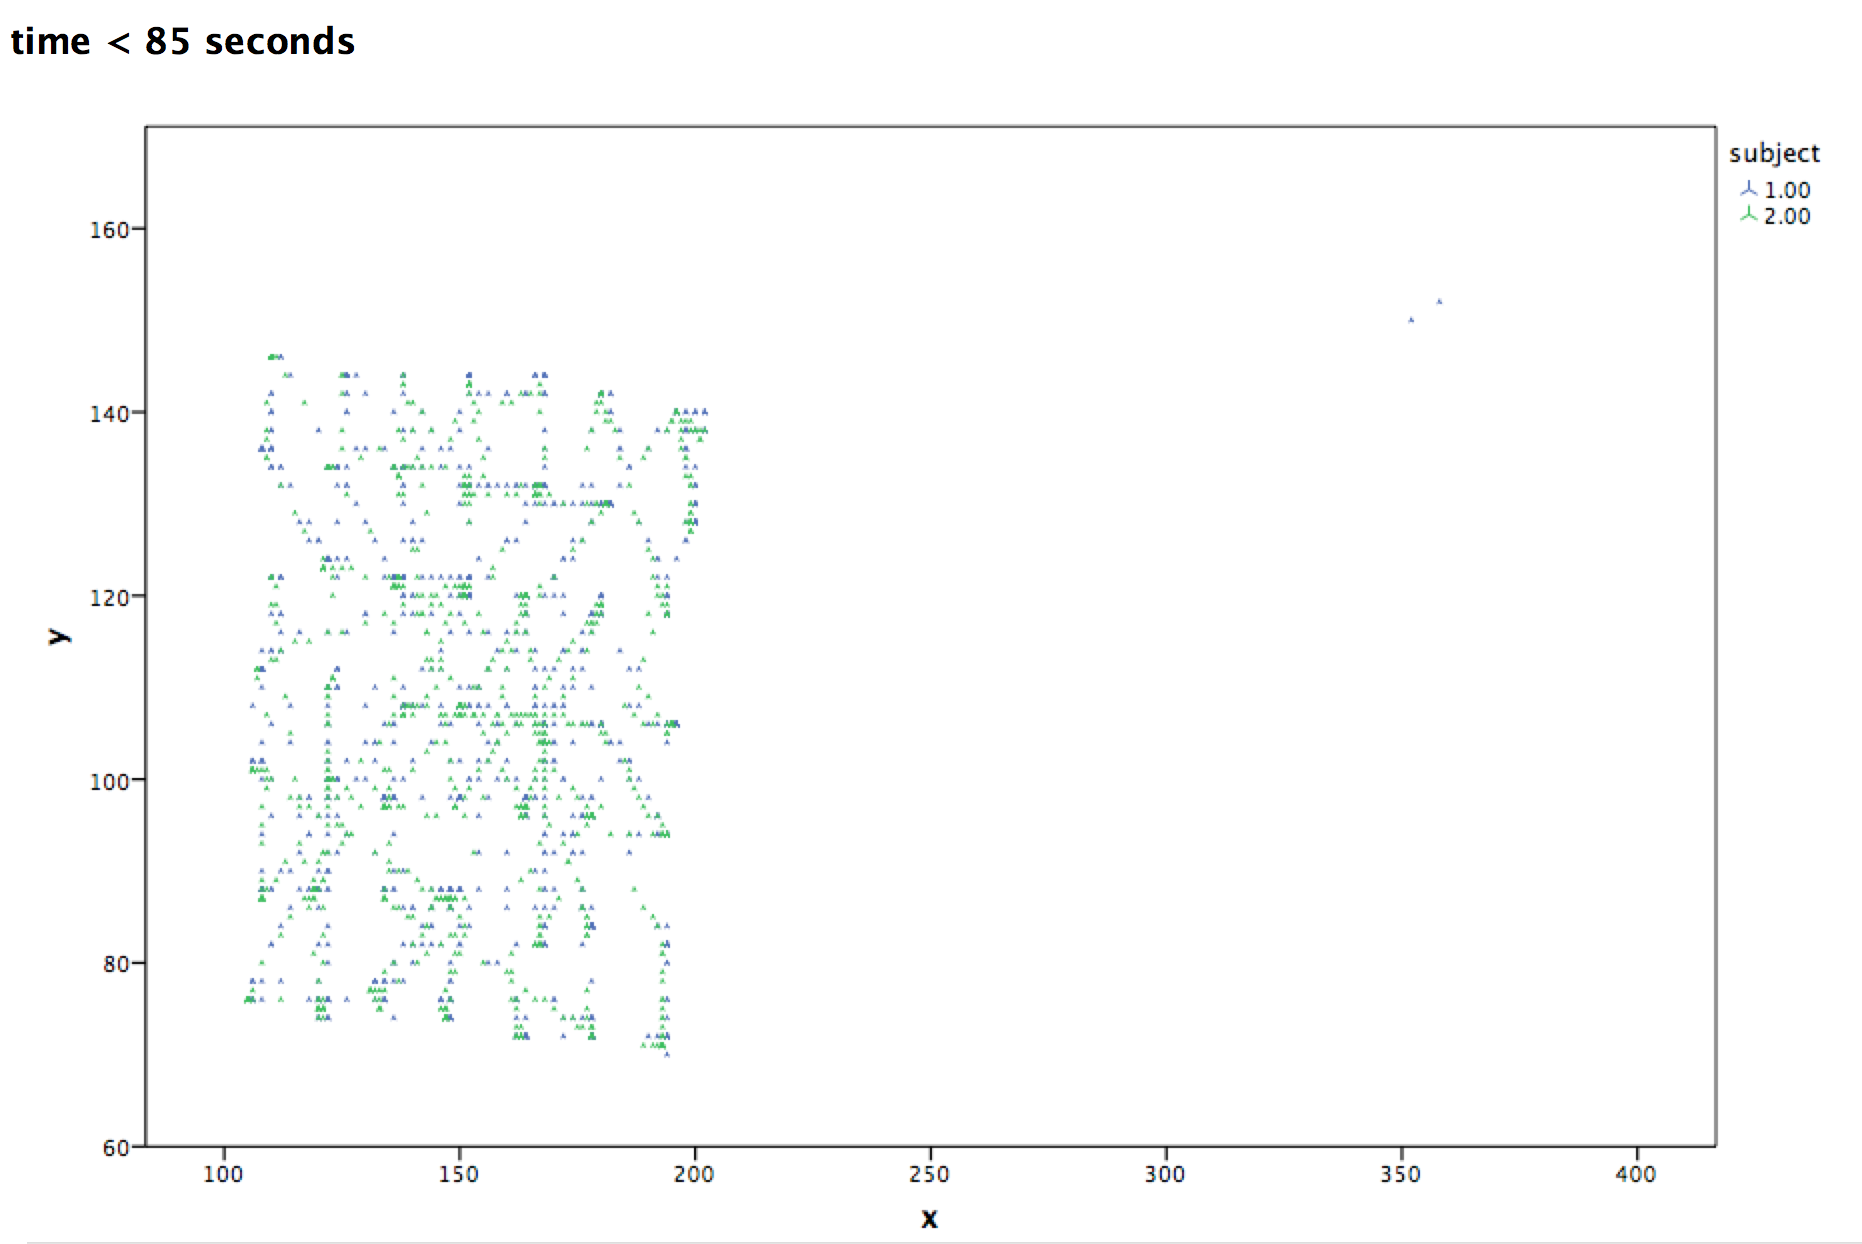
\includegraphics[scale=0.4]{./img/xy_first.png}

\noindent 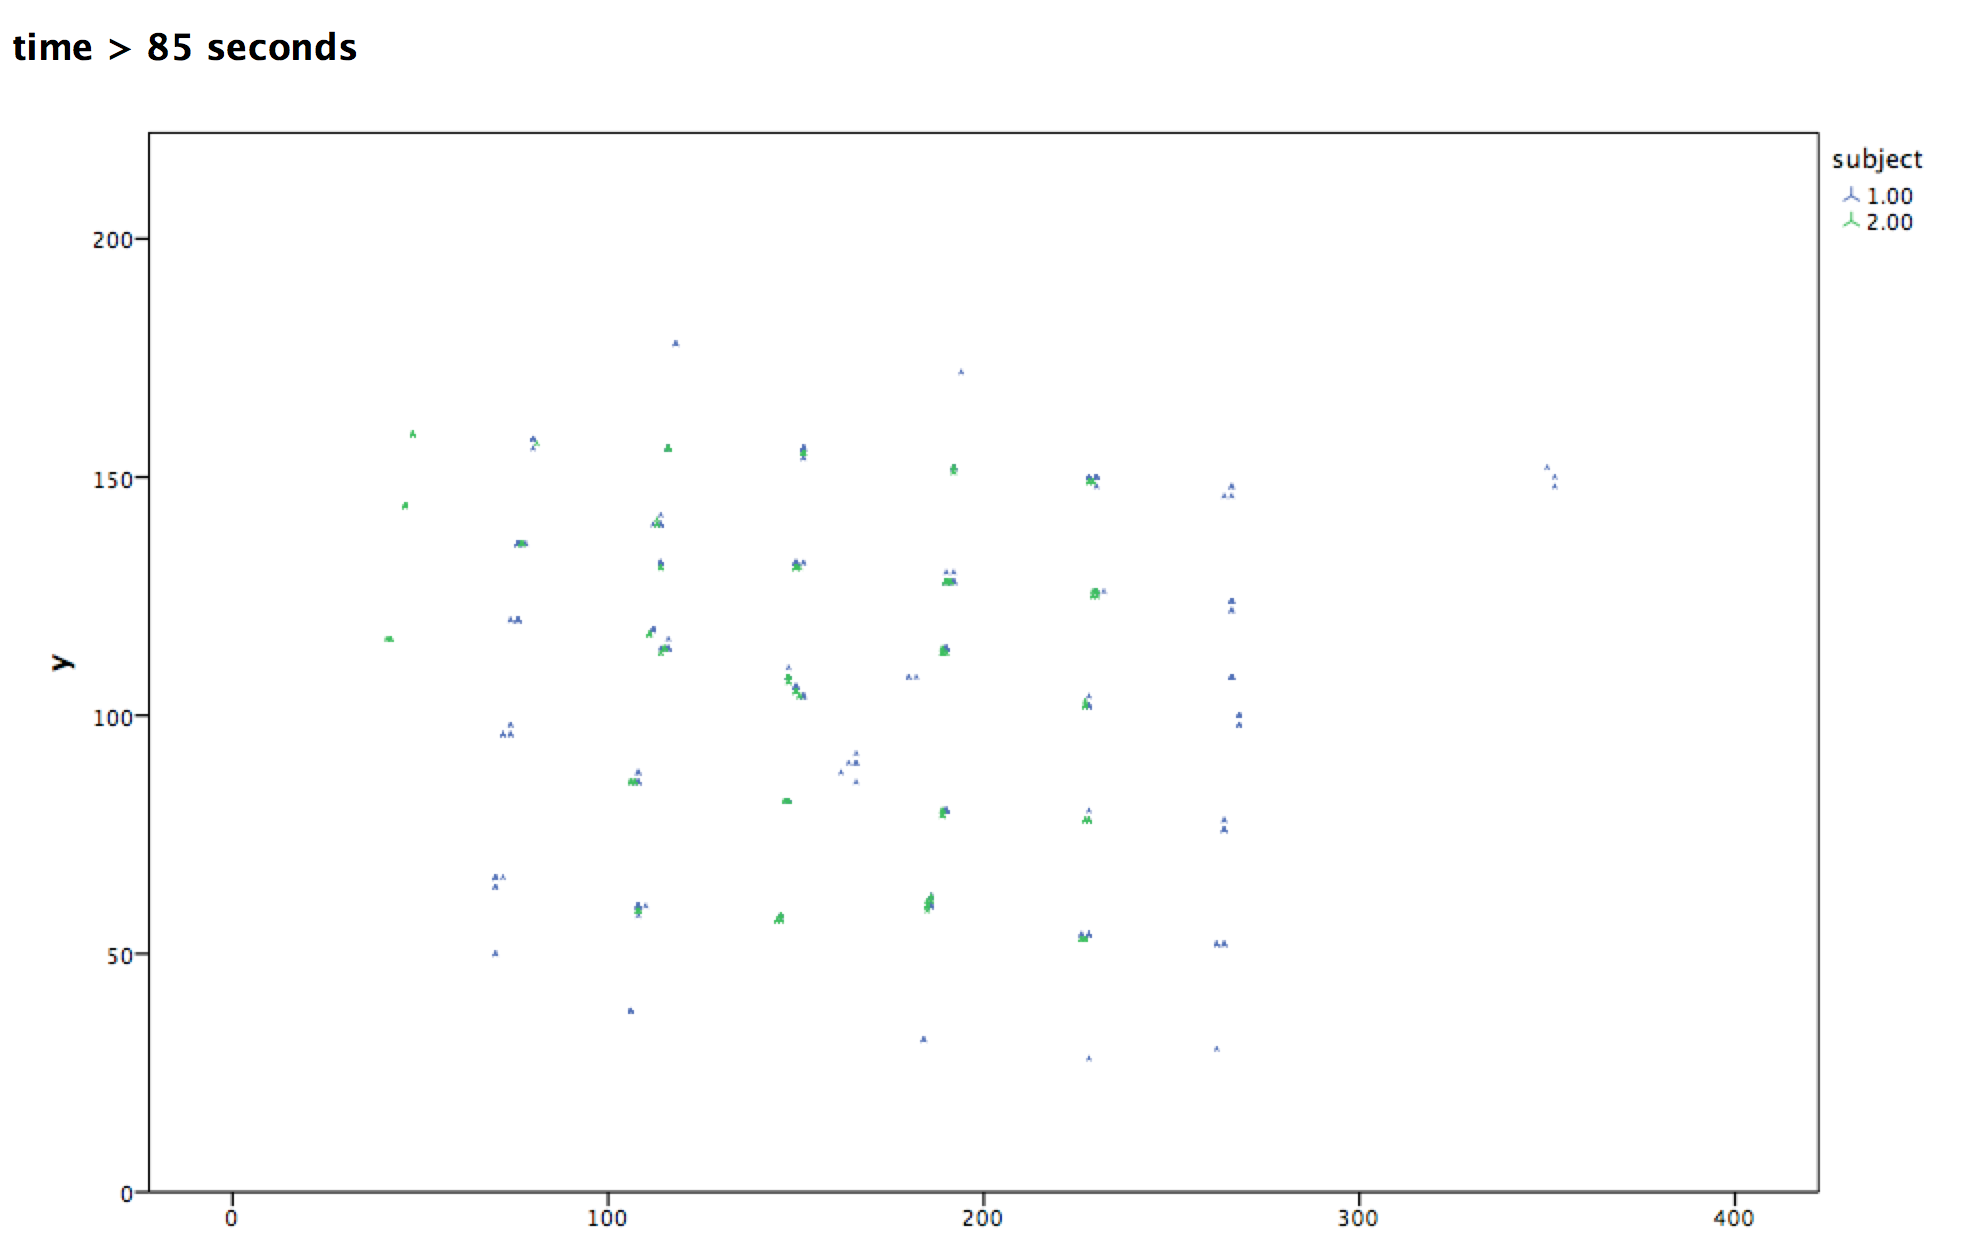
\includegraphics[scale=0.4]{./img/xy_last.png}

\noindent This is the x and y positions of where it's most lossy. There should be an array with 49 positions.\\
\end{document}